\chapter{Multi-Model Data}
\label{multimodel}

In the past, applications have tended to use mainly relational databases as their preferred way of storing data.
This has been in large part due to the lack of maturity in the multi-model data ecosystem, which has slowly been changing in recent years.
While sticking to a single data model (relational for example) has many benefits in terms of uniformity of modeling, access and management, in some use cases, it may be desirable to leverage the unique advantages offered by the usage of multiple different data models.
Testament to this is the number of multi-model database technologies on the rise in both academia and industry settings.
Among these are polystores~\cite{polystores}\cite{polystores2} (database systems consisting of multiple heterogeneous integrated database systems) and multi-model database systems~\cite{multimodel_dbs}\cite{multimodel_dbs2} (database systems supporting the storage of multiple data models at the same time).
While both of the mentioned multi-model options allow multi-model querying, neither provides a unified querying experience which would allow the user to ignore the specifics of the given models.
Altogether, we can broadly describe this trend towards using multi-model data as the NoSQL movement~\cite{nosql}.

The biggest advantage of using multiple data models within an application is the possibility of modeling the data in the most appropriate way possible, meaning being able to for example model graph data using graph structures, rather than having to reshape the data to conform to a different model.
Along with that, this approach can bring performance benefits, as databases suited to a particular model are naturally faster at storing and retrieving data in its native model~\cite{unibench}.

This chapter introduces the most popular data models, and showcases why one may want to use them to model their data.
It is important to understand the need for multi-model data before we delve deeper into the contents of this thesis, whose usefulness hinges on the fact that multi-model data is omnipresent in today's database ecosystem.

When talking about multi-model data, it can also be useful to have a unified vocabulary, since the terminology can differ between different data models.
Such a unification was proposed by Pavel Koupil in his 2022 dissertation~\cite{koupil_thesis}, and is shown in~\cref{table:datamodels:terms}.
There, we can see a set of unifying terms which cover the terminology of various popular models, for example the term \textit{kind} is used to refer to tables in relational data, collections in document data, or column families in columnar data.
This thesis uses this unifying terminology in multiple places, so it is recommended that the reader is familiar with these terms before moving on.

\begin{table}[ht]%!
\centering
\scriptsize
\caption{Unification of terms in popular models, proposed by Pavel Koupil~\cite{koupil_thesis}}
\label{table:datamodels:terms}
\def\arraystretch{1.5}
\begin{tabular}{
    >{\raggedright\arraybackslash}p{13.0mm} % suma = 145mm
    >{\raggedright\arraybackslash}p{15.2mm} % relational
    >{\raggedright\arraybackslash}p{15.7mm} % array
    >{\raggedright\arraybackslash}p{11.7mm} % graph
    >{\raggedright\arraybackslash}p{12.2mm} % rdf
    >{\raggedright\arraybackslash}p{16.2mm} % key/value
    >{\raggedright\arraybackslash}p{15.5mm} % document
    >{\raggedright\arraybackslash}p{11.7mm} % column
    }
        \toprule
        \textbf{Unifying term} & \textbf{Relational}  & \textbf{Array}        & \textbf{Graph}      & \textbf{RDF}            & \textbf{Key/Value}      & \textbf{Document}        & \textbf{Column}      \\
        \midrule
        Kind          & Table       & Matrix       & Label      & Set of triples & Bucket         & Collection      & Column family \\
        
        Record        & Tuple         & Cell         & Node / edge  & Triple         & Pair (key, value) & Document        & Row           \\
        
        Property      & Attribute   & Attribute    & Property   & Predicate      & Value          & JSON Field / XML element or attribute           & Column        \\
        Array         & --         & --          & Array      & --            & Array            & JSON array / repeating XML elements           & Array         \\
        Structure     & --         & --          & --        & --            & Set / ZSet / Hash            & Nested document & Super column \\
        Domain        & Data type   & Data type    & Data type  & IRI / literal / blank node & --            & Data type       & Data type     \\
        Value         & Value       & Value        & Value      & Object         & Value          & Value           & Value         \\
        Identifier    & Key & Coordinates & Identifier & Subject        & Key            & JSON identifier / XML ID or key      & Row key    \\
        Reference     & Foreign key & --          & --        & --            & --            & JSON reference / XML keyref       & --           \\
        \bottomrule
    \end{tabular}
\end{table}

\section{Aggregate-Oriented Models and Aggregate-Ignorant Models}

Before delving into the specifics of the various data models, we should note a major divide among how the data models behave.
They can be divided into two main camps.

The first one is aggregate-oriented models, which generally store and operate on aggregates -- data units with complex and often nested structure. 
Aggregate-oriented models generally focus on manipulating aggregates with various operations.
Database systems working with aggregates can use the aggregate boundaries to determine which bits of data will be manipulated together, which can be useful for sharding or replication.
As a result, cross-aggregate operations may be inefficient, or in some cases, totally impossible while maintaining Atomicity, Consistency, Isolation and Durability (ACID).
Examples of aggregate-oriented models include document, column-family, and key-value models.

In contrast, aggregate-ignorant models do not have a universal strategy of drawing aggregate boundaries, as these boundaries depend on how we manipulate the data.
This can be an advantage in the absence of a primary structure for accessing and manipulating the data, as it allows one to easily work with the data in different ways.
Examples of aggregate-ignorant models include relational and graph models.

\section{Relational Model}

Relational data is arguably the oldest data model which is widely used today~\cite{codd}.
Whenever one is designing a system which requires some sort of data persistence, relational databases are usually among the first options to be examined.
This is in large part due to their great track record of being solid, tested and well-understood by many.

Data in the relational model is organized into tables, with each table having a rigid schema defined by a set of columns, and data being stored in the form of table rows.
The relational model generally contains some kind of key or identifier for each table row, be it a simple or compound one.
An example of relational data can be seen in~\cref{fig:relationaldata}, where it is shown in the form of an ER diagram~\cite{er} on the left, and in its native representation on the right.

\begin{figure}[h]
\centering
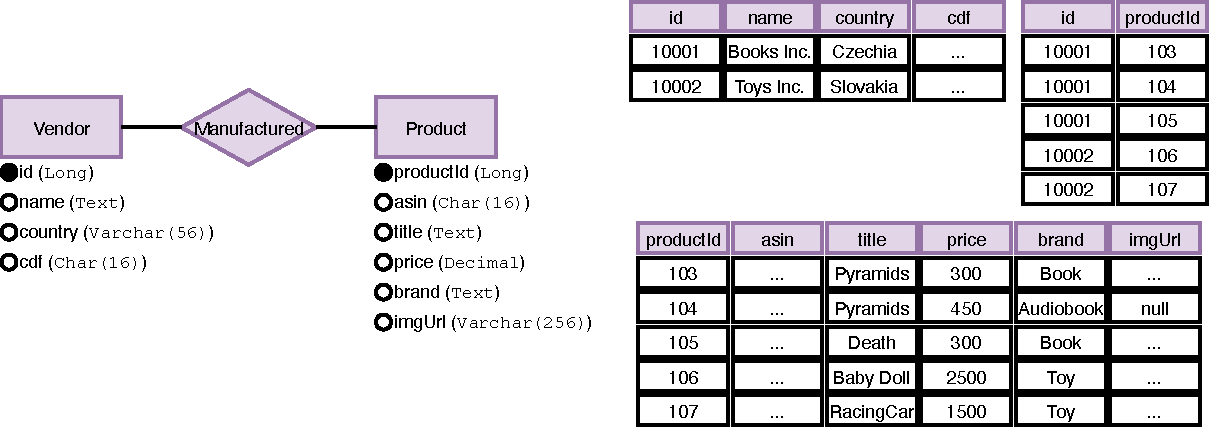
\includegraphics[scale=0.66]{img/example-relational.pdf}
\caption{An example of relational data~\cite{inference}.}
\label{fig:relationaldata}
\end{figure}

When querying relational data (typically using SQL), the largest amount of effort is generally spent on joining data together using database joins, in order to extract the data from the normalized form that it is stored in.
This is a tradeoff which many are happy to make, considering relational databases generally offer great support for Online Transactional Processing (OLTP) workloads in the form of transactions -- bundles of database commands which are executed with "all or none" semantics.
Relational systems also tend to have very good support of database integrity management tools, allowing database administrators to have full confidence in the continued integrity of their data.

However, the NoSQL movement has brought with it a desire for database \textit{horizontal scalability}, as use cases arise where simply vertically scaling a relational database system by improving its hardware is not always enough~\cite{relational_out}.
In such use cases brought on by the advent of Big Data, many are seeking to leverage the benefits of traditional relational databases in the context of scalable and highly available data.
This has spawned efforts which can be described as the NewSQL movement~\cite{newsql}.
As examples, one can look at databases like CockroachDB\footnote{\url{https://www.cockroachlabs.com/product/}} or VoltDB\footnote{\url{https://www.voltactivedata.com/}}, which offer relational databases with the speed and scalability of NoSQL systems.

For the purposes of this thesis, it is necessary to point out a few representative database system for each data model, for the purposes of developing a universal querying approach.
It would not be reasonably feasible to develop such an approach with respect to every database from each data model, therefore we simply select a couple of popular representative systems which feature the main characteristics of its corresponding data model.
For relational databases, we put forward PostgreSQL\footnote{\url{https://www.postgresql.org/}} and MySQL\footnote{\url{https://www.mysql.com/}} as some of the most popular options.

\section{Document Model}

One of the main critiques often leveraged at relational databases, especially by developers who highly value speed of development, is the fact that they can have a prohibitively high start-up cost in terms of data modeling and database management.
If speed of development and ease of reasoning about the data model are of high importance, one may soon find themselves considering document oriented databases~\cite{document_dbs}.
These databases are aggregate-oriented, with the aggregate boundaries being drawn as the boundaries of \textit{documents} -- self-contained pieces of data with a potentially complex structure.
We can think of documents in a document-oriented database in terms of objects in a programming language -- each has a structure and carries some data.
Objects in the document-oriented model generally do not need to adhere to a schema, which makes document databases popular where ease of development is paramount.
An example of document data may be seen in~\cref{fig:documentdata}.

\begin{figure}[ht]
\centering
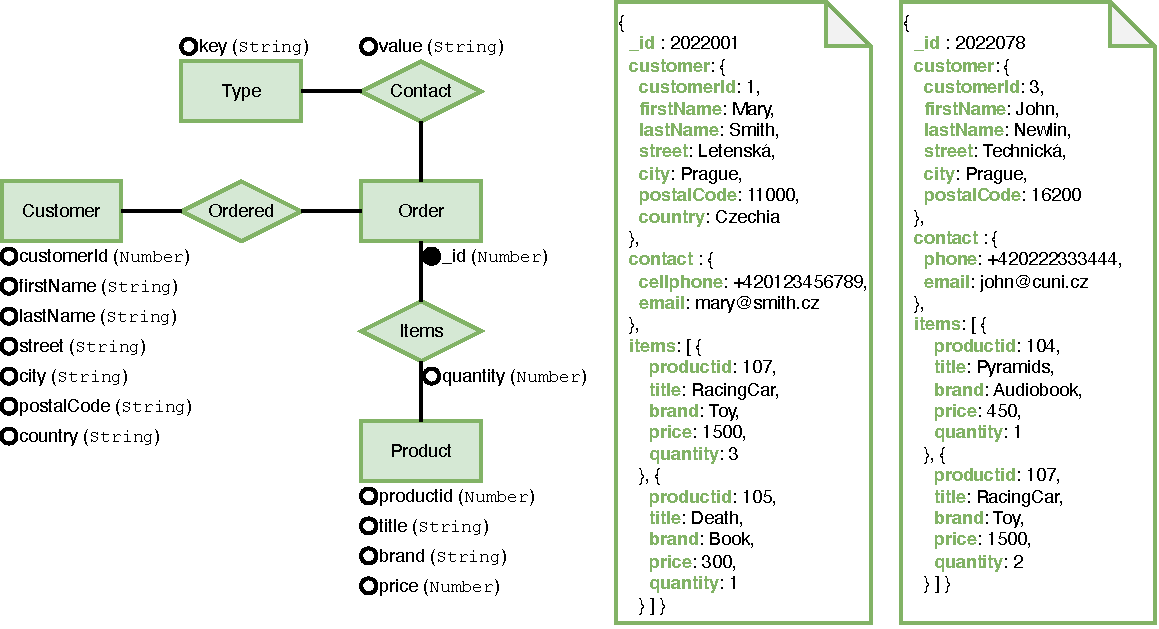
\includegraphics[scale=0.66]{img/example-json.pdf}
\caption{An example of document data in the JSON format~\cite{inference}.}
\label{fig:documentdata}
\end{figure}

Choosing a representative of the document model is not difficult, as MongoDB\footnote{\url{https://www.mongodb.com/}} is a very prominent and popular document database, which is very widely used in practice.
MongoDB organizes documents into \textit{collections}, which are sets of related documents which may be queried together.
Working with MongoDB can have a relatively user-friendly learning curve, as one can store objects from most popular programming languages into the database in JSON\footnote{\url{https://www.json.org/json-en.html}} form without too many modifications, unlike the relational model where Object-Relational Mappers (ORM) are often required.
However, in more complex use cases where working with multiple documents in a single transaction is required, developers may find the complexity resurfacing.

\section{Graph Model}

Graph databases model data in terms of objects (nodes) and relationships between those objects.
There exist two main kinds of graph models -- edge-labeled graphs and property graphs.
Both of these graph models are discussed at greater length in~\cref{querylanguages:section:graphdatamodels}.
To see an example of data in the graph model, we refer the reader to~\cref{fig:graphdata}.

\begin{figure}[h]
\centering
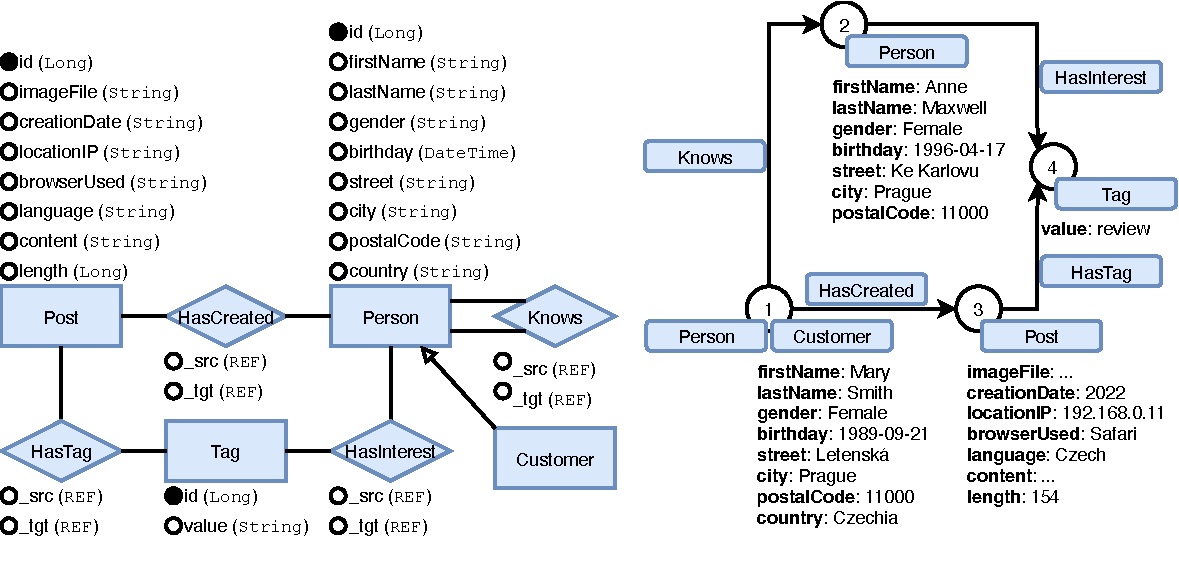
\includegraphics[scale=0.66]{img/example-graph.pdf}
\caption{An example of graph data~\cite{inference}.}
\label{fig:graphdata}
\end{figure}

In general, graph databases are best suited for use cases where the graph nature of the data is important.
These systems excel at querying for relationships between objects, and at finding patterns in the data.
Unlike relational data, relationships in graph data models are first-class entities, and may often be given properties.
In theory, graph databases provide a performance advantage compared to relational databases when considering graph-oriented workloads, however, this is not a clear-cut point of consensus in the academic community~\cite{against_graph}.

Regardless of performance implications however, it is undeniable that when presented with graph-like data, it is most convenient to model that data in a graph database.
As such, a number of graph databases have reached wide adoption today.
One of the foremost representatives of graph databases is Neo4j\footnote{\url{https://neo4j.com/}}.
Although the rest of this thesis considers Neo4j as the main representative of graph databases, a special mention should be made to RDF data which is briefly discussed in~\cref{querylanguages:subsection:edgelabeled}, as RDF is also a graph data format, and is often used in the semantic web community.

\section{Wide-Column Model}

Wide-column data may seem very similar to relational data on the surface -- both have concepts like rows and columns, storing data in table-like structures.
However, the major difference from the relational model is the fact that the names and format of the columns may differ between rows of the same table (or column family, as it is sometimes called).
Column-oriented databases store data in column-major order rather than in row-major order, meaning all values for a single column are stored contiguously, rather than contiguously storing all values for a single row.
This confers performance benefits in many cases, such as for workloads where reading all data related to a single record is rare.
An example of columnar data is shown in~\cref{fig:columnardata}.

\begin{figure}[hb]
\centering
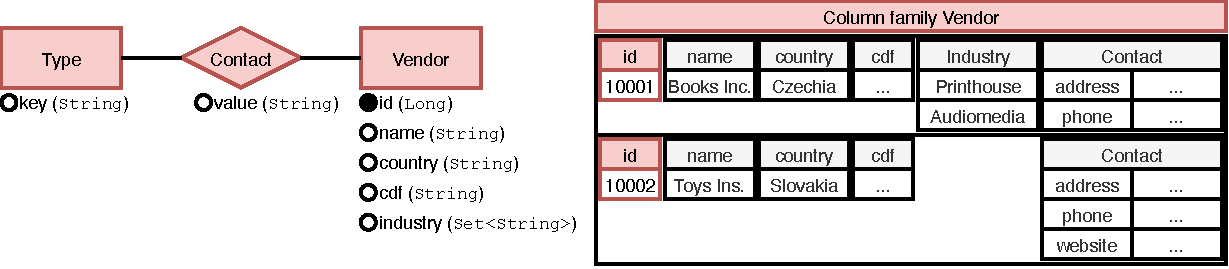
\includegraphics[scale=0.66]{img/example-columnar.pdf}
\caption{An example of columnar data~\cite{inference}.}
\label{fig:columnardata}
\end{figure}

When picking a representative for wide-column databases, Apache Cassandra\footnote{\url{https://cassandra.apache.org/_/index.html}} is a clear candidate, as it is open-source and widely used.

\section{Key-Value Model}

A key-value database or key-value store may be thought of as a hash table, which is designed to quickly store and retrieve opaque values.
As such, key-value databases are very well suited to workloads like caching, often times being used as an in-memory cache of a slower, on-disk database.
Naturally, the weakness of key-value databases is the fact that they are not generally designed to examine or query the actual values stored in any way beyond retrieving them based on the key.
Therefore, they may not be ideal for more complex transactional or analytical workloads.
See~\cref{fig:keyvaluedata} for an example of key-value data.

\begin{figure}[ht]
\centering
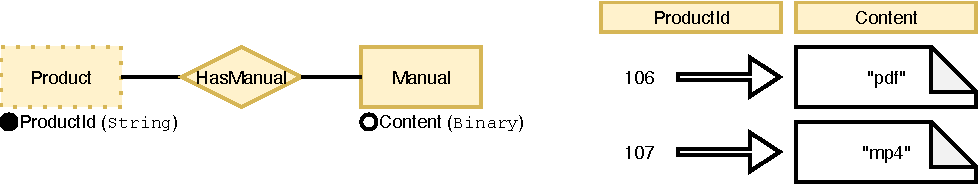
\includegraphics[scale=0.66]{img/example-keyval.pdf}
\caption{An example of key-value data~\cite{inference}.}
\label{fig:keyvaluedata}
\end{figure}

We will consider Redis\footnote{\url{https://redis.io/}} and Riak KV\footnote{\url{https://riak.com/products/riak-kv/}} as representatives of a key-value stores for the purposes of this thesis.
